\section{Probability}
\subsection{Probability density function (PDF)}
The area below the graph between point $A$ and $B$ shows the probability. Therefore:
\[
\int_{-\infty}^{\infty}\varphi(x)dx = 1
\]

\subsection{Continuous cumulative distribution (CDF)}
The CDF $F$ shows probability of an event to occur:
\[
\varphi(x) = F'(x) \xRightarrow[]{} \int_{-\infty}^{x}\varphi(\zeta)d\zeta = F_x(x)
\]
$F$ is the Stammfunktion of PDF $\varphi$.


\subsection{Normal distribution}
\[
\varphi(x|\mu, \sigma) = \frac{1}{\sigma\sqrt{2\pi}}e^{-\frac{(x-\mu)^2}{2\sigma^2}}
\]
With help of the ML-Prinzip ($\prod_{k = 1}^{n}\varphi(x_k|\mu, \sigma)$) chapter \ref{ml} we can estimate the parameters
\begin{align*}
	\mu &= \frac{1}{n}\sum_{k=1}^{n}x_k &\qquad 	\sigma^2 &= \frac{1}{n}\sum_{k=1}^{n}(x_k - \mu)^2
\end{align*}

\subsection{Maximum Likelihood}\label{ml}
This is often used as cost function for finding optimum values for parameters.
\[
L(\theta) = \prod_{i = 1}^{n}f(y_i, \theta)
\]

For ML and other application the negative log likelihood function is used:
\[
L(\theta) = -\ln\left( \prod_{i = 1}^{n}f(y_i, \theta)\right) = -\sum_{i=1}^{n}\ln(f(y_i; \theta))
\]

\subsection{Random Numbers}
Statistically independent random numbers
\[
f_Y(y) =f_X(x) \cdot \frac{dx}{dy}
\]

\subsection{Unif Function}
Continuous uniform distribution (unif)

PDF
\[
\text{unif}(x| a,b) = \begin{cases}
	\frac{1}{b-a} & a \le x \le b \\
	0 & \text{else}
\end{cases}
\]

CDF
\[
\int\text{unif}(x| a,b)dx = \begin{cases}
	0 & x \le a \\
	\frac{x-a}{b-a} & a \le x \le b \\
	1 & \text{else}
\end{cases}
\]
\begin{center}
	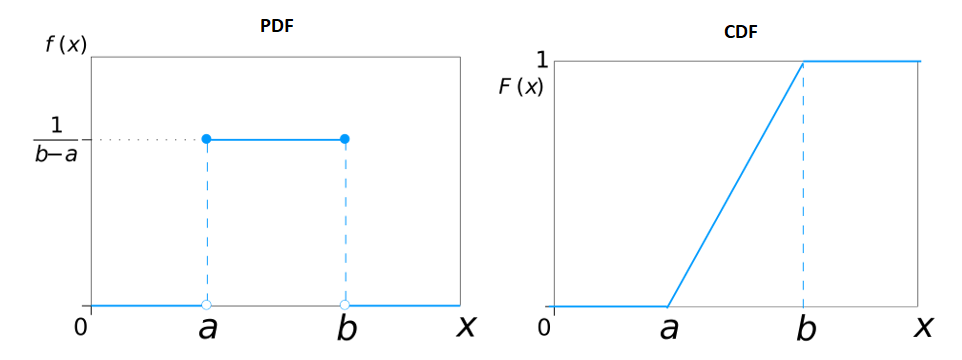
\includegraphics[width=0.8\columnwidth]{Images/unif}
\end{center}